% !TEX program = xelatex
% vim:foldmethod=marker:foldmarker=<<<,>>>
\documentclass[compress]{beamer}

%<<< Preamble
\usepackage[english]{babel}
\usepackage{metalogo}
\usepackage{listings}
\usepackage{fontspec}
\usepackage{amsmath, amssymb}
\usepackage{stackrel}
\usepackage{tikz}
\usepackage{svg}
\usepackage{unicode-math}
\usepackage{subcaption}
\usepackage[theme=nord,charsperline=60,linenumbers]{jlcode}

\usetheme{Nord}

\setmainfont{Roboto}
% \setsansfont{DejaVu Serif}
% \setmonofont{CaskaydiaCove Nerd Font Mono}
\setmonofont{JuliaMono}


\makeatletter
\def\verbatim@nolig@list{}
\newcommand\pin{%
\parbox[t]{10pt}{\raisebox{0.2pt}{\usebeamercolor[fg]{mybullet}{$\ast$}}}}
\makeatother

\newcommand{\E}[1]{\ensuremath{E\left\{#1\right\}}}
\newcommand{\norm}[1]{\ensuremath{\lVert#1\rVert}}

\hypersetup{
    colorlinks=true,
    urlcolor=NordBlue
}

\DeclareMathOperator*{\argmax}{argmax}
\DeclareMathOperator*{\Var}{Var}

\AtBeginDocument{
    \fontsize{8}{12}
    \selectfont

}

\AtBeginSection[]
{
    \begin{frame}[c,noframenumbering,plain]
        \tableofcontents[sectionstyle=show/hide,subsectionstyle=show/show/hide]
    \end{frame}
}


\AtBeginSubsection[]
{
    \begin{frame}[c,noframenumbering,plain]
        \tableofcontents[sectionstyle=show/hide,subsectionstyle=show/shaded/hide]
    \end{frame}
}
%>>>

\title{Project I: Apertures}
\subtitle{}
\author{\Large Simon Andreas Bjørn}
\date{\large March 8, 2023}

\begin{document}

\begin{frame}[plain,noframenumbering]
    \maketitle
\end{frame}

\begin{frame} % <<< Unfocused ASA Simulation
    \frametitle{Unfocused ASA Simulation}
    We want to run the \texttt{ASA.m} and inspect the results.
    Running the \texttt{ASA.m} code yields the following to plots
    \begin{columns}
        \begin{column}{0.5\textwidth}
            \begin{figure}
                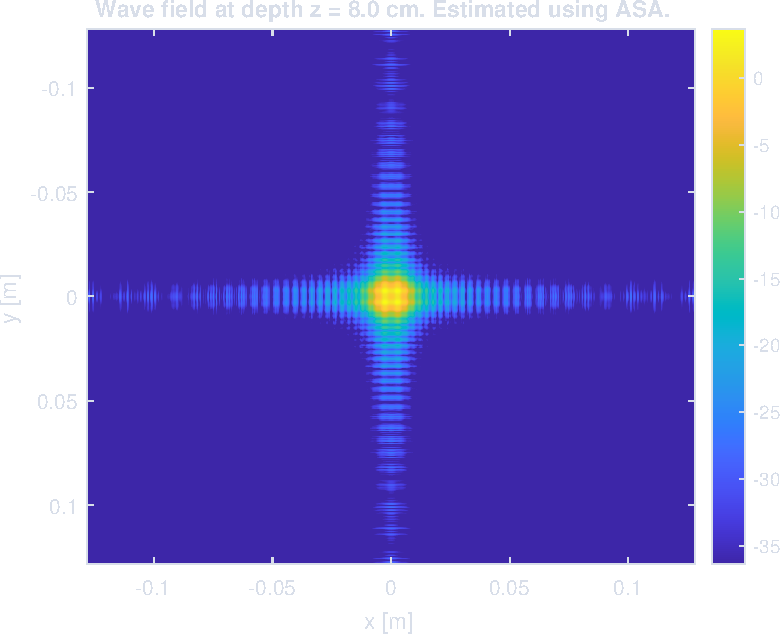
\includegraphics[height=0.5\textheight]{"../1a.pdf"}
            \end{figure}
        \end{column}
        \begin{column}{0.5\textwidth}
            \begin{figure}
                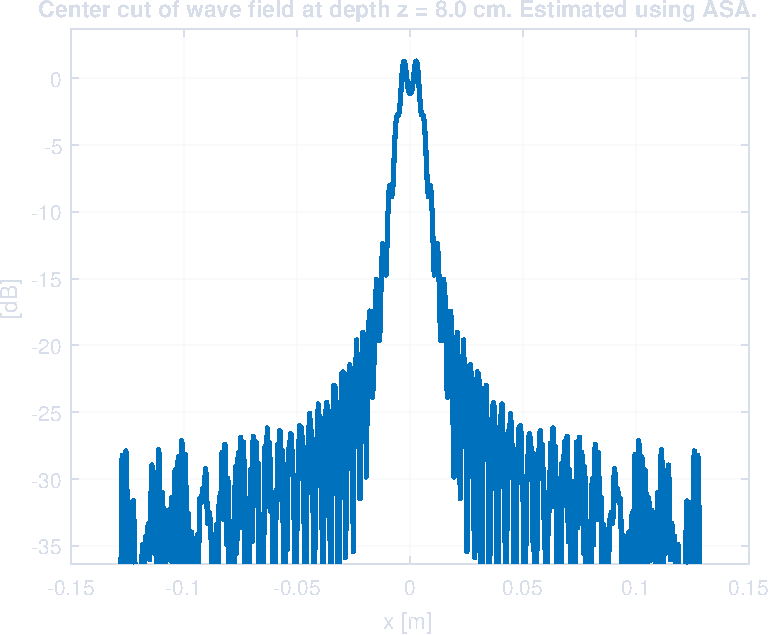
\includegraphics[height=0.5\textheight]{"../1b.pdf"}
            \end{figure}
        \end{column}
    \end{columns}
    \begin{itemize}
        \item Left plot is the wave field $U(x,y,z=z_0)$, of a uniform square point source with $D=15\lambda$
        \item Right plot is the pressure along the x-axis at $y = 0, z=z_0$.
    \end{itemize}
    The wave field has propagated a minimal amount from the true source at $z=0$.
\end{frame} % >>>

\begin{frame}[fragile] % <<< Unfocused ASA Simulation 2
    \frametitle{Unfocused ASA Simulation 2}
    We want to taper the propagator, and propagate the wave field for some distance $z=0.4$.
    Modifying the \texttt{ASA.m} script with the additions written in the assignment text,
    I have the following plots and code
    \begin{columns}
        \begin{column}{0.5\textwidth}
            \begin{figure}
                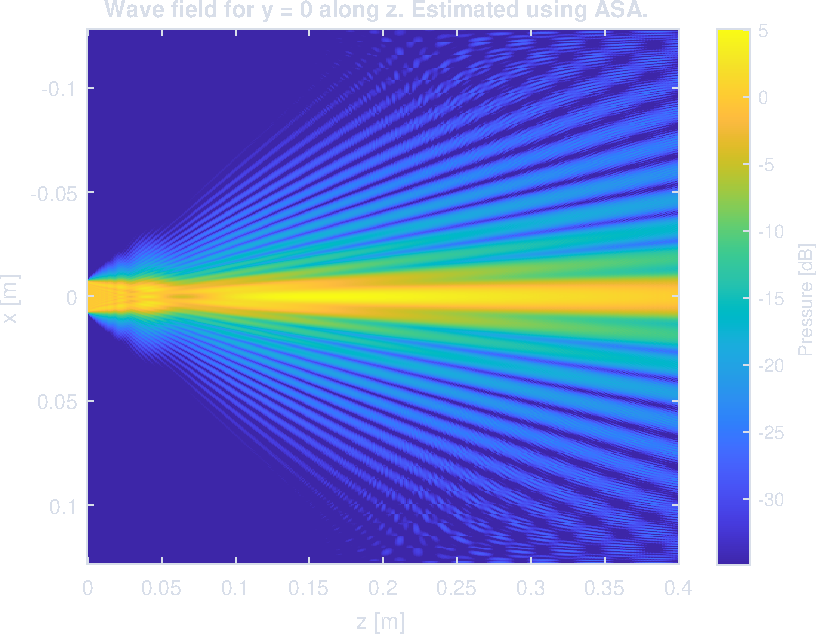
\includegraphics[width=\columnwidth]{"../2a.pdf"}
            \end{figure}
        \end{column}
        \begin{column}{0.5\textwidth}
            \begin{figure}
                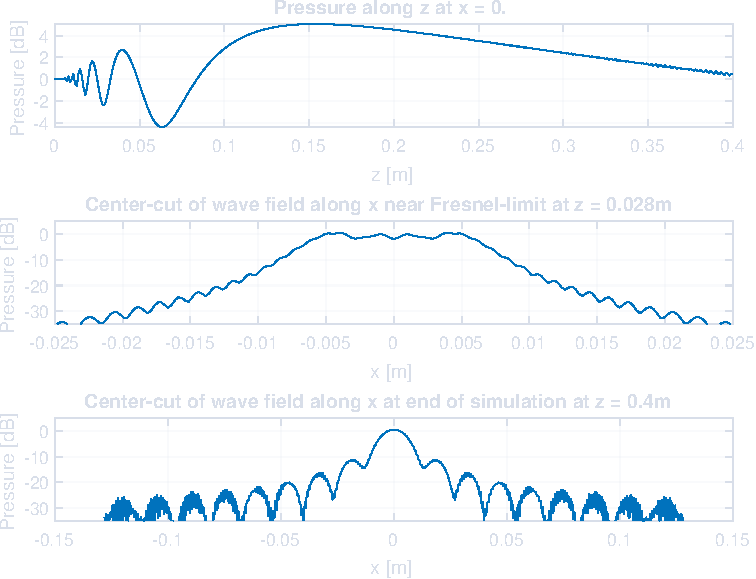
\includegraphics[width=\columnwidth]{"../2b.pdf"}
            \end{figure}
        \end{column}
    \end{columns}
    \vspace{1mm}
    For the near field, I chose the Fresnel-limit
    at $d_F = \frac{D^2}{4λ} \approx 0.028m$. We see a clear difference between the
    wave field at the Fresnel-limit and in the far field.
\end{frame}
% >>>

\begin{frame}[fragile] % <<< Array Pattern - Grating lobes
    \frametitle{Array Pattern - Grating lobes}
    Given an array of $M=24$ elements, we want to find the beampattern of the array
    with different spacings of the elements. Here I use the \texttt{beampattern.m} code.
    \begin{columns}
        \begin{column}{0.52\textwidth}
            \begin{jllisting}[gobble=16, language=Matlab]
                DXs = [P.lambda/4   P.lambda/2 ...
                       P.lambda   2*P.lambda];

                ks = linspace(-1,1,N);
                kx = 2*pi/P.lambda*ks;
                weights = ones(M, 1);

                for dx_idx = 1:numel(DXs)
                    dx = DXs(dx_idx);
                    D = M*dx;
                    xpos = linspace(-D/2, D/2, M);
                    
                    W = beampattern(xpos, kx, weights);
                end
            \end{jllisting}
        \end{column}
        \begin{column}{0.5\textwidth}
            \begin{figure}
                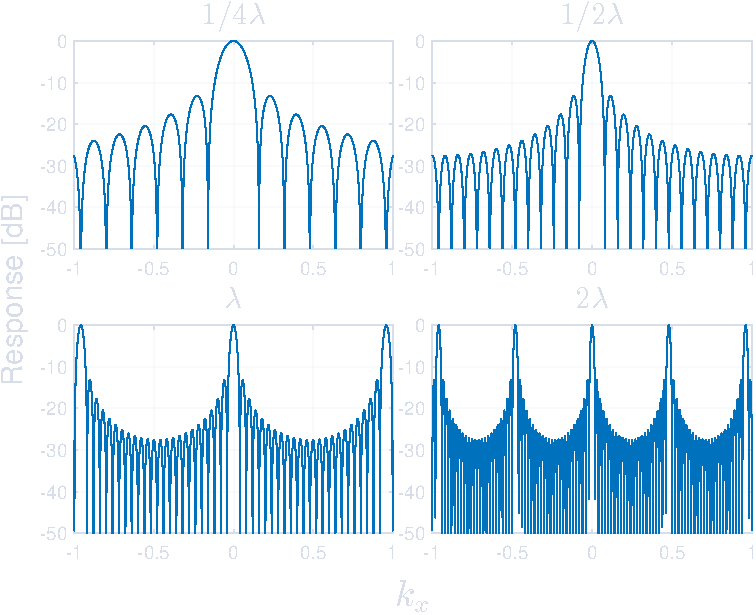
\includegraphics[width=\columnwidth]{"../4.pdf"}
            \end{figure}
        \end{column}
    \end{columns}
    We see that for element distance $D \le \frac{λ}{2}$ we don't see any grating lobes,
    while for $D \ge \frac{λ}{2}$ we see the grating lobes appear at the end of the array
    pattern.
\end{frame}
% >>% >>>

\begin{frame}[fragile] % <<< Element weighting and spacing
    \frametitle{Element weighting and spacing}
    We now want to apply a temper to the array, using a Kaiser windo and see how
    different windows impact the array pattern.
    
    Applying the window is pretty streight forward
    \begin{enumerate}
        \item Create a window of given length and shape
        \item Normalize window so sum of elements are 1
        \item Apply temper to beampattern
    \end{enumerate}

    \begin{jllisting}[gobble=8,language=Matlab]
        beta = betas(beta_idx);
        win = kaiser(M, beta);
        norm_win = win / sum(win(:));
        W = beampattern(xpos, kx, norm_win);
    \end{jllisting}
    Using {\texttt analyzeBP.m} we log the mainlobe width at -3dB and -6dB, as
    well as the max height of the sidelobes.
\end{frame}
% >>>

\begin{frame} % <<< Element weighting and spacing 2
    \frametitle{Element weighting and spacing 2}
    We also want to find the white noise gain of the array.
    Since we use a normalized kaiser window, we assume that
    $W^Ha\left(\omega,\tau\right) = 1$ which gives the gain
    $ GW\left(\theta\right)=\norm{\vec{w}}^{-2} $. Plotting the results from
    our logged values we have the following
    \begin{columns}
        \begin{column}{0.5\textwidth}
            \begin{figure}
                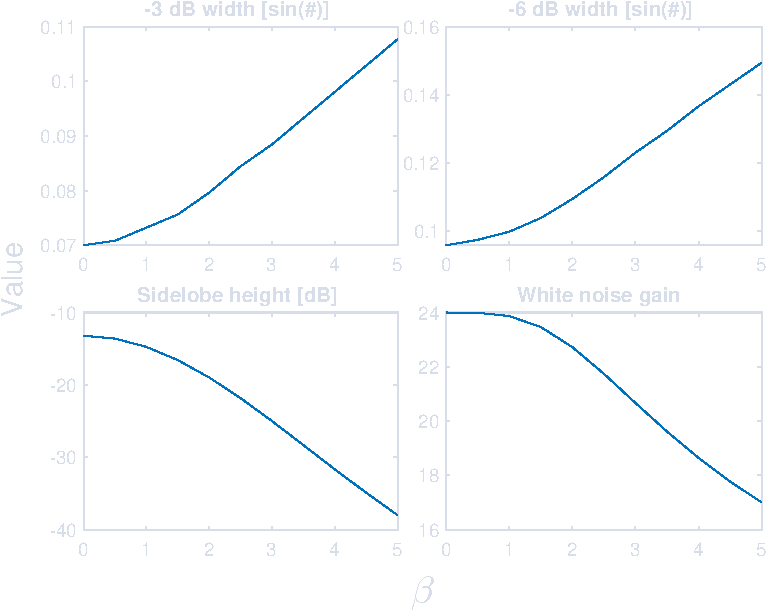
\includegraphics[width=\columnwidth]{"../5.pdf"}
            \end{figure}
        \end{column}
        \begin{column}{0.5\textwidth}
            Looking at the plot to the left, we see that 
            \begin{itemize}
                \item Increasing beta increases width of mainlobe
                \item Suppresses the height of the sidelobes
                \item Decreases the white noise gain
            \end{itemize}
        \end{column}
    \end{columns}
    Conclusion there is a trade-off when using the temper. It supresses the 
    sidelobes to some degree at the cost of angular resolution.
\end{frame}
% >>>





\end{document}
